Although the FE discretization of the QGE is relatively scarce, the
corresponding error analysis seems to be even more scarce. To our knowledge,
\emph{all} the error analysis for the FE discretization of the QGE has been
done for the vorticity-streamfunction formulation, none being done for the
streamfunction formulation. Furthermore, to the best of our knowledge, all the
available error estimates for the FE discretization of the QGE are
\emph{suboptimal}. The first FE error analysis for the FE discretization of
the QGE was carried out by Fix \cite{Fix}, in which suboptimal error estimates
for the vorticity-streamfunction formulation were proved. Indeed, relationships
(4.7) and (4.8) (and the discussion above these) in \cite{Fix} show that the FE
approximations for \emph{both} the potential vorticity (denoted by $\zeta$) and
streamfunction (denoted by $\psi$) consist of piecewise polynomials of degree
$k-1$. At the top of page 381, the author concludes that the error analysis
yields the following estimates:
\begin{eqnarray}
  \| \psi - \psi^h \|_1 &=& O(h^{k-1}), \label{eqn:fix_1} \\
  \| \zeta - \zeta ^h \|_0 &=& O(h^{k-1}) . \label{eqn:fix_2}
\end{eqnarray}
Although the streamfunction error estimate \eqref{eqn:fix_1} appears to be
optimal, the potential vorticity error estimate \eqref{eqn:fix_2} is clearly
suboptimal. Indeed, using piecewise polynomials of degree $k-1$ for the FE
approximation of the vorticity, one would expect an $O(h^k)$ error estimate in
the $L^2$ norm. Medjo \cite{Medjo99, Medjo00} used a FE discretization of the
vorticity-streamfunction formulation and proved error estimates for the time
discretization, but no error estimates for the spatial discretization. Finally,
Cascon et al. \cite{Cascon} proved both \emph{a priori} and \emph{a posteriori}
error estimates for the FE discretization of the \emph{linear Stommel-Munk}
model (see Section~\ref{ch:Tests} for more details). This model, while similar
to the QGE, has one significant difference: the linear Stommel-Munk model is
linear, whereas the QGE is nonlinear.
%Thus, it appears that \emph{no optimal} error estimates for the FE
%discretization of the QGE exist.

We note that the state-of-the-art in the FE error analysis for the QGE seems to
reflect the FE error analysis for the \emph{two-dimensional Navier-Stokes
equations (2D NSE)}, to which the QGE are similar in form.  Indeed, as carefully
discussed in \cite{Gunzburger89}, the 2D NSE in streamfunction-vorticity
formulation are easy to implement (only $C^0$ elements are needed for a
conforming discretization), but the available error estimates are suboptimal
(see Section 11.6 in \cite{Gunzburger89}).
\begin{remark}
  It must be noted that although QGE and NSE look quite similar in their
  streamfunction forms, they are quite different. A significant difference lies
  in the asymmetry introduced by the $\beta$-term, $\dfrac{\partial
  \psi}{\partial x}$. This $\beta$-term introduces the Coriolis effect and
  differentiates the western boundary from the eastern boundary.  As the Rossby
  number, $Ro$ decreases the effect of the Coriolis becomes more and more
  significant. As displayed in \autoref{fig:NSEnotQGE} the stronger the
  Coriolis force (smaller $Ro$) the narrower the western boundary layer becomes.
  Additionally, we see that in the two gyre forcing seen in
  \autoref{fig:NSEnotQGE} as $Ro$ decreases the distance between the gyres
  decreases, creating an internal boundary layer. Both these facts lend to
  precautions that must be taken into account when implementing the QGE, which
  are not necessary in the implementation of the NSE.
  %Thus, stabilization methods for the NSE may not work as well for the QGE.
\end{remark}

\begin{figure}
  \begin{center}
  \begin{subfigure}{0.4\textwidth}
    \centering
    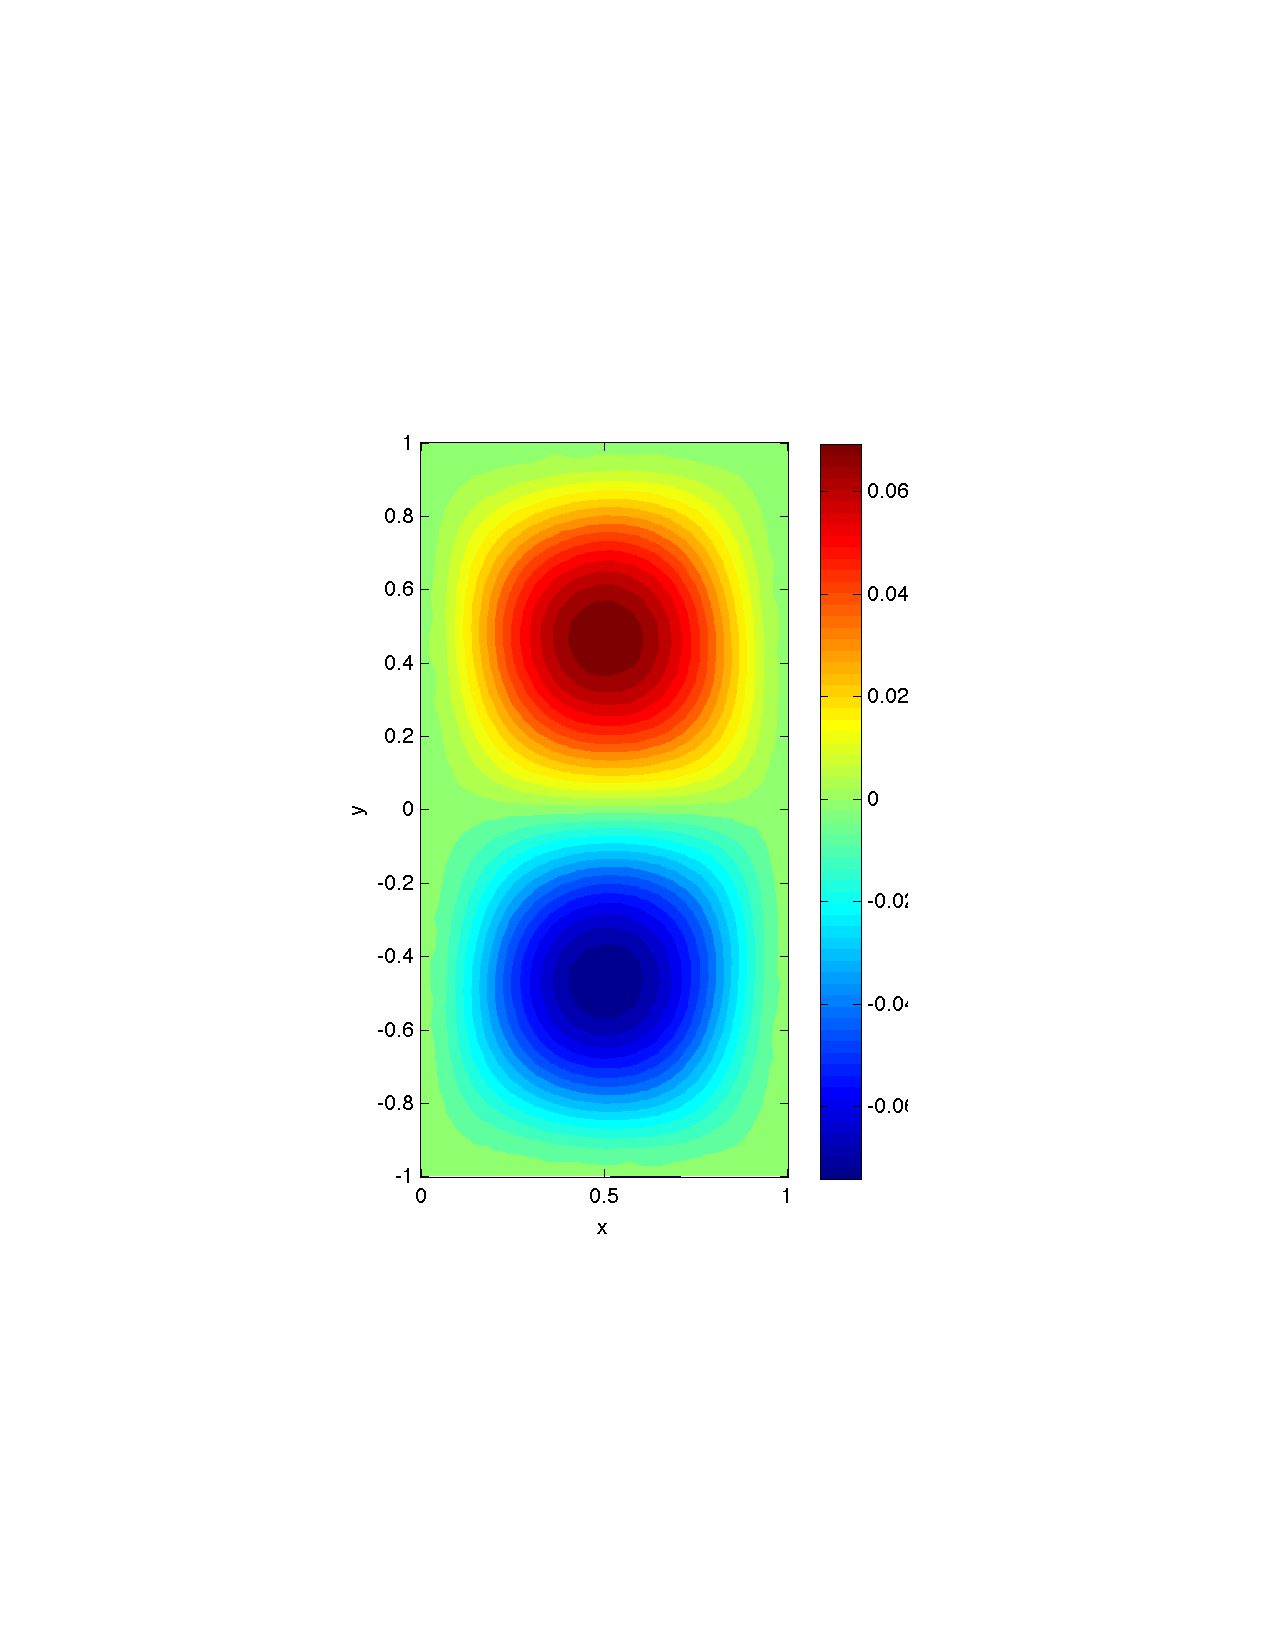
\includegraphics[scale=0.5]{Figures/Re200h16k1000}
    \caption{NSE}
    \label{sfi:NSE}
  \end{subfigure}
  \begin{subfigure}{0.4\textwidth}
    \centering
    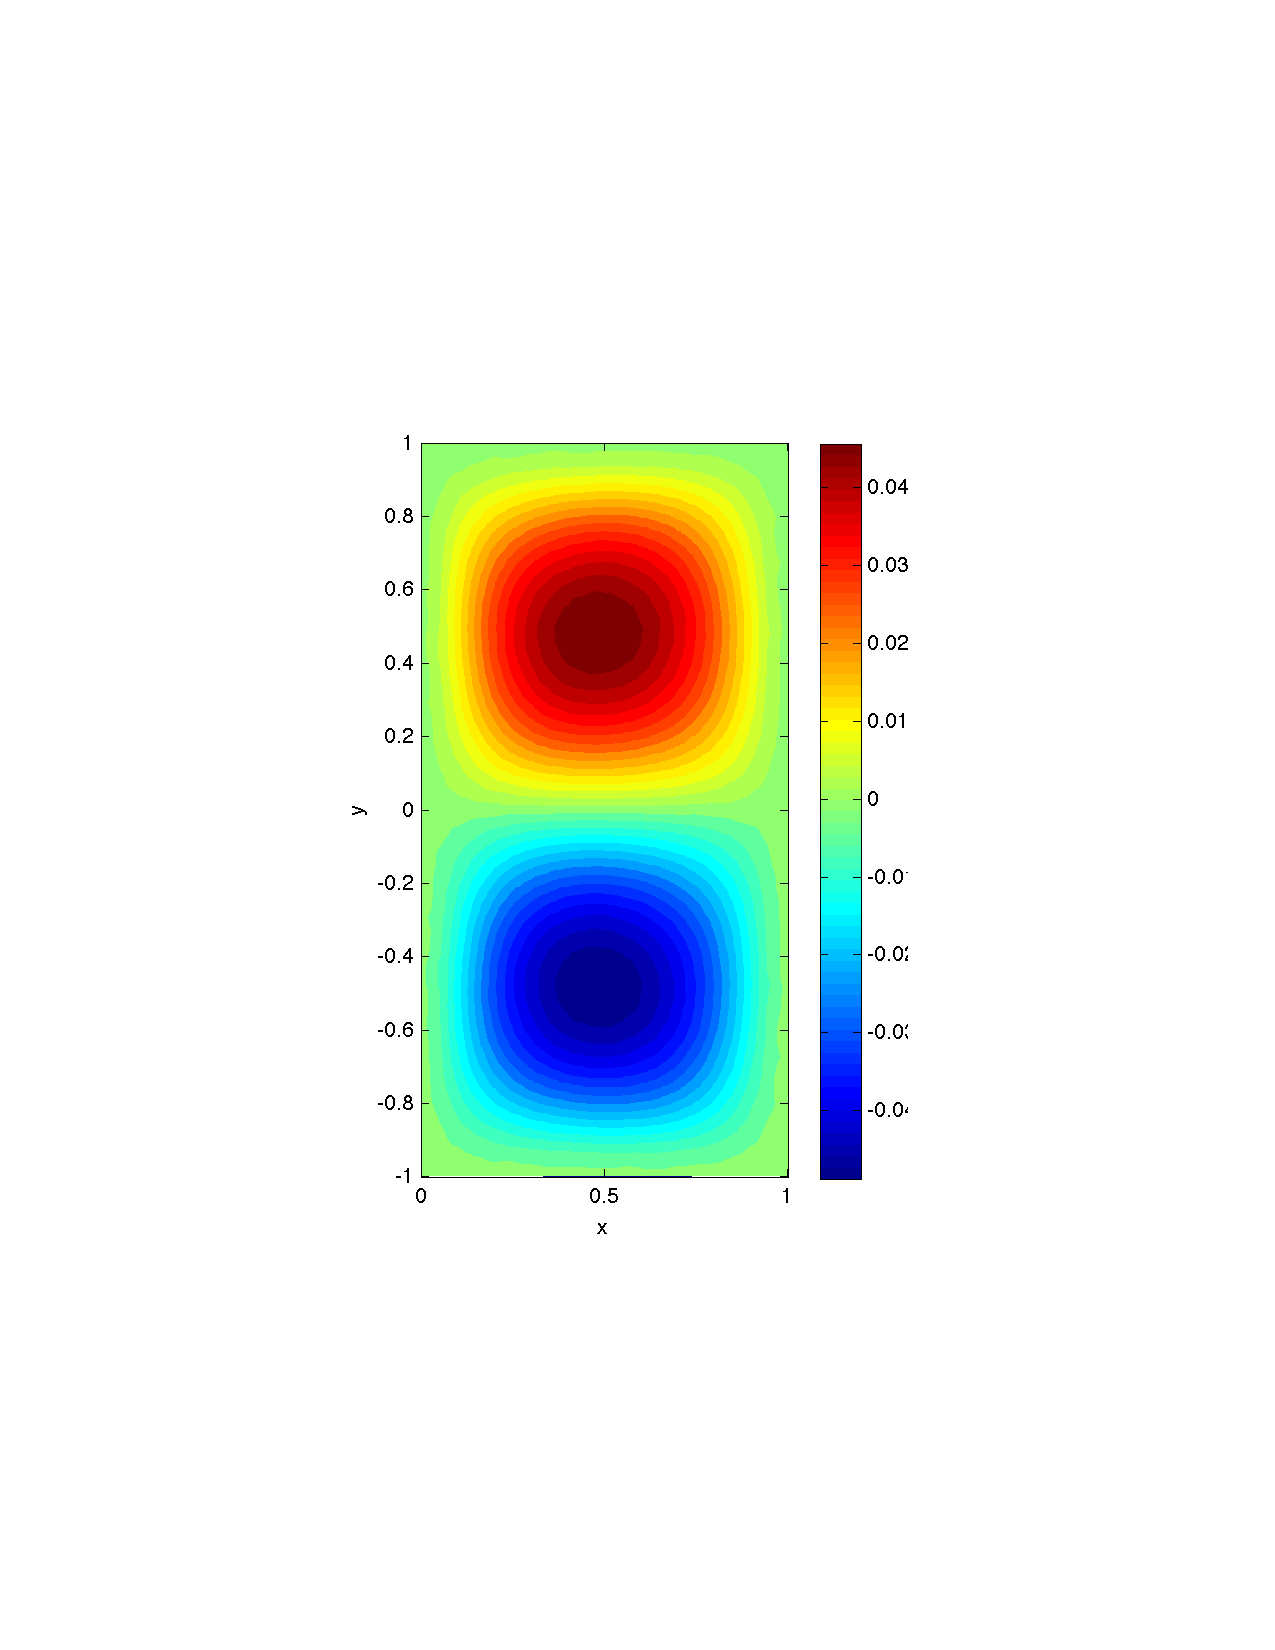
\includegraphics[scale=0.5]{Figures/Re200Ro1h16k1000}
    \caption{QGE, $Ro=1$}
    \label{sfi:QGERo1}
  \end{subfigure}
  \begin{subfigure}{0.3\textwidth}
    \centering
    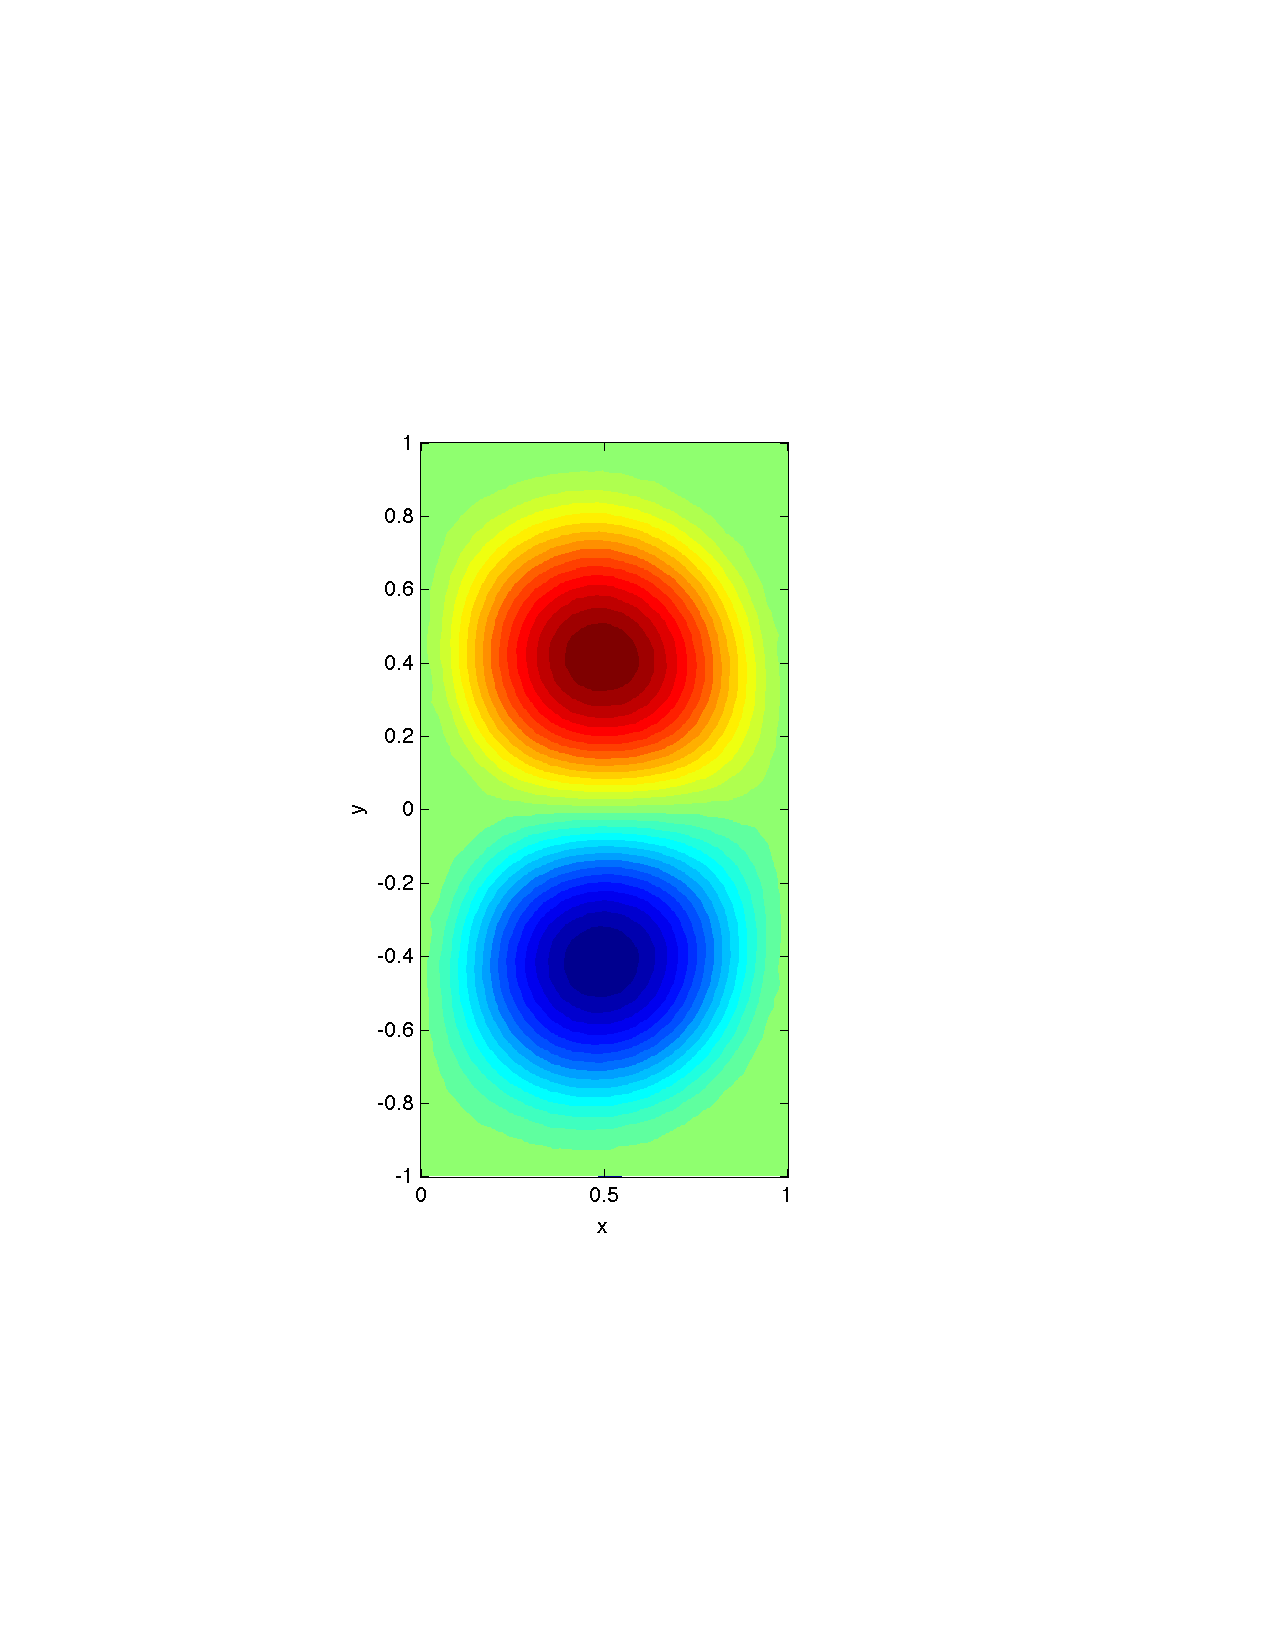
\includegraphics[scale=0.5]{Figures/Re200Ro1E-1h16k1000}
    \caption{QGE, $Ro=0.1$}
    \label{sfi:QGERo0.1}
  \end{subfigure}
  \begin{subfigure}{0.3\textwidth}
    \vspace{1.3em}
    \centering
    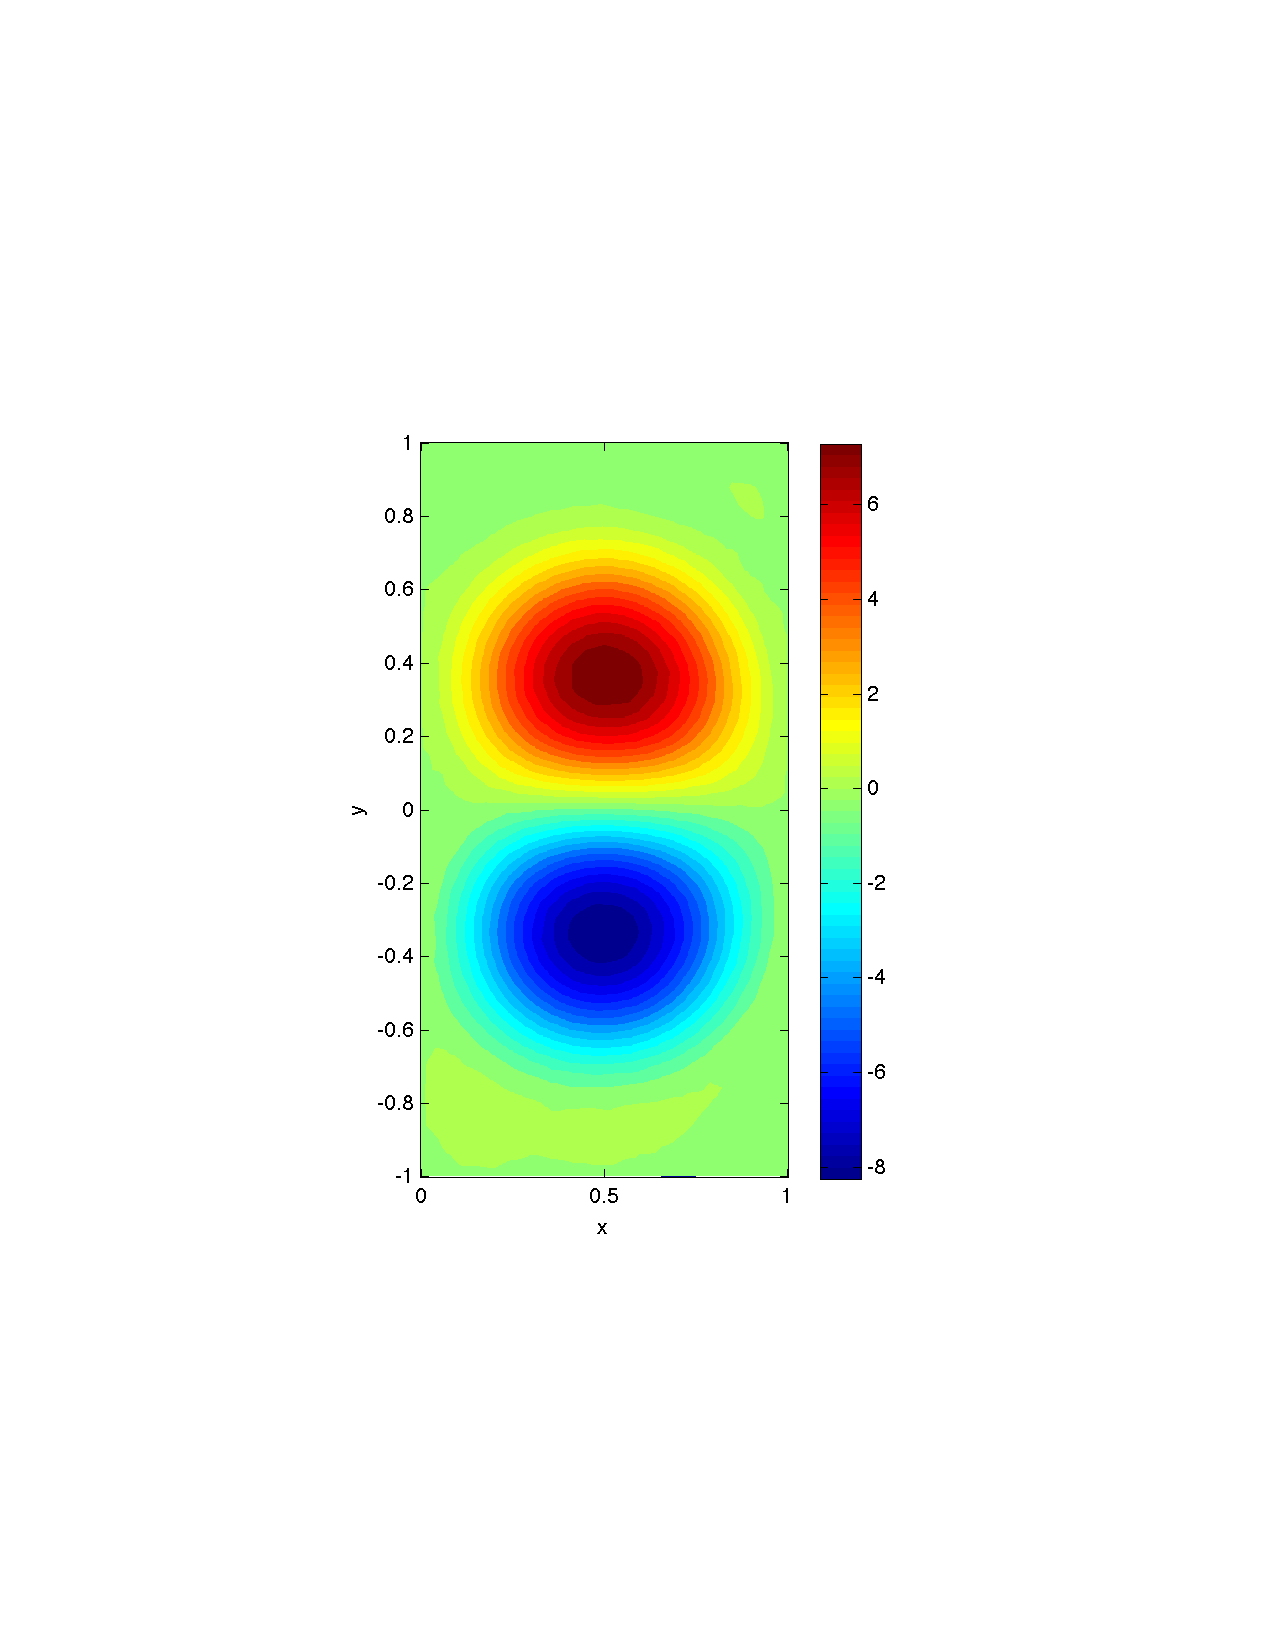
\includegraphics[scale=0.5]{Figures/Re200Ro1E-2h16k1000}
    \label{sfi:QGERo0.01}
    \caption{QGE, $Ro=0.01$}
  \end{subfigure}
  \begin{subfigure}{0.3\textwidth}
    \centering
    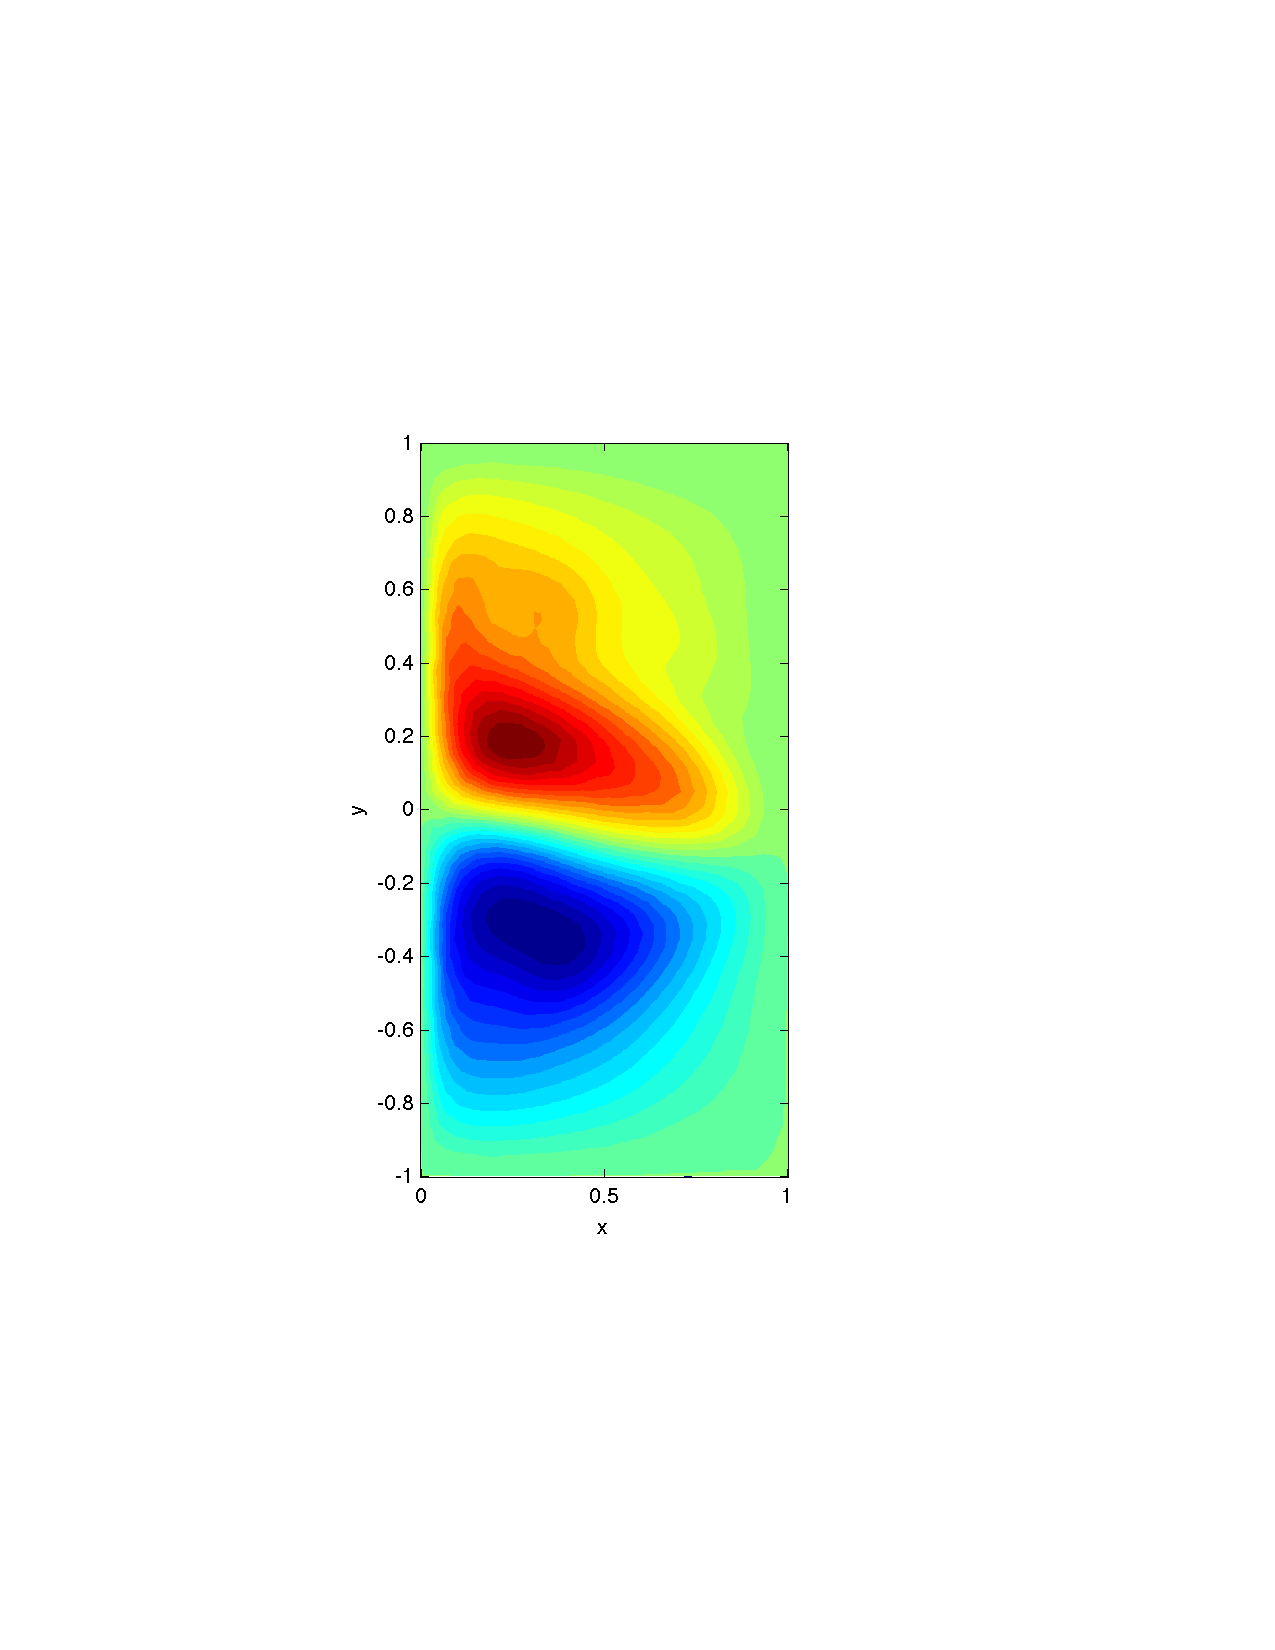
\includegraphics[scale=0.5]{Figures/Re200Ro1E-3h16k1000}
    \caption{QGE, $Ro=0.001$}
    \label{sfi:QGERo0.001}
  \end{subfigure}
  \caption{QGE is not NSE: Time averaged streamfunctions, time interval $0\le t
    \le 10$ time step $dt=1\times 10^{-3}$, Reynolds number $Re= 200$, forcing
    term $F = \sin (\pi y)$.}
  \label{fig:NSEnotQGE}
  \end{center}
\end{figure}

Next, we summarize the discussion in \cite{Gunzburger89},
since we believe it sheds light on the QGE setting. For $C^0$ piecewise
polynomial of degree $k$ FE approximation for \emph{both} the vorticity
(denoted by $\omega$) and streamfunction (denoted by $\psi$), the error
estimates given in \cite{Girault86} are (see (1.26) in \cite{Gunzburger89}):
\begin{eqnarray}
  | \psi - \psi^h |_1 + \| \omega - \omega^h \|_0 \leq C \, h^{k - 1/2} \, | \ln h |^{\sigma} ,
  \label{eqn:gunzburger_1}
\end{eqnarray}
where $\sigma = 1$ for $k = 1$ and $\sigma = 0$ for $k > 1$. It is noted in
\cite{Gunzburger89} that the error estimate in \eqref{eqn:gunzburger_1} is not
optimal: one may loose a half power in $h$ for the derivatives of the
streamfunction (i.e., for the velocity), and three-halves power for the
vorticity. It is also noted that there is computational and theoretical evidence
that \eqref{eqn:gunzburger_1} is not sharp with respect to the streamfunction
error. Furthermore, in \cite{Fix84} it was shown that, for the \emph{linear}
Stokes equations, the derivatives of the streamfunction are essentially
optimally approximated (see (11.27) in \cite{Gunzburger89}):
\begin{eqnarray}
  | \psi - \psi^h |_1 \leq C \, h^{k - \varepsilon} , \label{eqn:gunzburger_2}
\end{eqnarray}
where $\varepsilon = 0$ for $k > 1$ and $\varepsilon > 0$ is arbitrary for $k =
1$. That being said, it is then noted in \cite{Gunzburger89} that
\eqref{eqn:gunzburger_1} seems to be sharp for the vorticity error and thus
vorticity approximations are, in general, very poor.
